
%% bare_jrnl.tex
%% V1.4b
%% 2015/08/26
%% by Michael Shell
%% see http://www.michaelshell.org/
%% for current contact information.
%%
%% This is a skeleton file demonstrating the use of IEEEtran.cls
%% (requires IEEEtran.cls version 1.8b or later) with an IEEE
%% journal paper.
%%
%% Support sites:
%% http://www.michaelshell.org/tex/ieeetran/
%% http://www.ctan.org/pkg/ieeetran
%% and
%% http://www.ieee.org/

%%*************************************************************************
%% Legal Notice:
%% This code is offered as-is without any warranty either expressed or
%% implied; without even the implied warranty of MERCHANTABILITY or
%% FITNESS FOR A PARTICULAR PURPOSE!
%% User assumes all risk.
%% In no event shall the IEEE or any contributor to this code be liable for
%% any damages or losses, including, but not limited to, incidental,
%% consequential, or any other damages, resulting from the use or misuse
%% of any information contained here.
%%
%% All comments are the opinions of their respective authors and are not
%% necessarily endorsed by the IEEE.
%%
%% This work is distributed under the LaTeX Project Public License (LPPL)
%% ( http://www.latex-project.org/ ) version 1.3, and may be freely used,
%% distributed and modified. A copy of the LPPL, version 1.3, is included
%% in the base LaTeX documentation of all distributions of LaTeX released
%% 2003/12/01 or later.
%% Retain all contribution notices and credits.
%% ** Modified files should be clearly indicated as such, including  **
%% ** renaming them and changing author support contact information. **
%%*************************************************************************


% *** Authors should verify (and, if needed, correct) their LaTeX system  ***
% *** with the testflow diagnostic prior to trusting their LaTeX platform ***
% *** with production work. The IEEE's font choices and paper sizes can   ***
% *** trigger bugs that do not appear when using other class files.       ***                          ***
% The testflow support page is at:
% http://www.michaelshell.org/tex/testflow/



\documentclass[journal]{IEEEtran}
%
% If IEEEtran.cls has not been installed into the LaTeX system files,
% manually specify the path to it like:
% \documentclass[journal]{../sty/IEEEtran}





% Some very useful LaTeX packages include:
% (uncomment the ones you want to load)


% *** MISC UTILITY PACKAGES ***
%
%\usepackage{ifpdf}
% Heiko Oberdiek's ifpdf.sty is very useful if you need conditional
% compilation based on whether the output is pdf or dvi.
% usage:
% \ifpdf
%   % pdf code
% \else
%   % dvi code
% \fi
% The latest version of ifpdf.sty can be obtained from:
% http://www.ctan.org/pkg/ifpdf
% Also, note that IEEEtran.cls V1.7 and later provides a builtin
% \ifCLASSINFOpdf conditional that works the same way.
% When switching from latex to pdflatex and vice-versa, the compiler may
% have to be run twice to clear warning/error messages.






% *** CITATION PACKAGES ***
%
\usepackage{amsmath}
\usepackage{amssymb}
\usepackage{bm}
\usepackage{cite}
\usepackage{graphicx}
\usepackage{multirow} %表の列結合
\usepackage{booktabs} %表の罫線の太さ
% cite.sty was written by Donald Arseneau
% V1.6 and later of IEEEtran pre-defines the format of the cite.sty package
% \cite{} output to follow that of the IEEE. Loading the cite package will
% result in citation numbers being automatically sorted and properly
% "compressed/ranged". e.g., [1], [9], [2], [7], [5], [6] without using
% cite.sty will become [1], [2], [5]--[7], [9] using cite.sty. cite.sty's
% \cite will automatically add leading space, if needed. Use cite.sty's
% noadjust option (cite.sty V3.8 and later) if you want to turn this off
% such as if a citation ever needs to be enclosed in parenthesis.
% cite.sty is already installed on most LaTeX systems. Be sure and use
% version 5.0 (2009-03-20) and later if using hyperref.sty.
% The latest version can be obtained at:
% http://www.ctan.org/pkg/cite
% The documentation is contained in the cite.sty file itself.






% *** GRAPHICS RELATED PACKAGES ***
%
\ifCLASSINFOpdf
  % \usepackage[pdftex]{graphicx}
  % declare the path(s) where your graphic files are
  % \graphicspath{{../pdf/}{../jpeg/}}
  % and their extensions so you won't have to specify these with
  % every instance of \includegraphics
  % \DeclareGraphicsExtensions{.pdf,.jpeg,.png}
\else
  % or other class option (dvipsone, dvipdf, if not using dvips). graphicx
  % will default to the driver specified in the system graphics.cfg if no
  % driver is specified.
  % \usepackage[dvips]{graphicx}
  % declare the path(s) where your graphic files are
  % \graphicspath{{../eps/}}
  % and their extensions so you won't have to specify these with
  % every instance of \includegraphics
  % \DeclareGraphicsExtensions{.eps}
\fi
% graphicx was written by David Carlisle and Sebastian Rahtz. It is
% required if you want graphics, photos, etc. graphicx.sty is already
% installed on most LaTeX systems. The latest version and documentation
% can be obtained at:
% http://www.ctan.org/pkg/graphicx
% Another good source of documentation is "Using Imported Graphics in
% LaTeX2e" by Keith Reckdahl which can be found at:
% http://www.ctan.org/pkg/epslatex
%
% latex, and pdflatex in dvi mode, support graphics in encapsulated
% postscript (.eps) format. pdflatex in pdf mode supports graphics
% in .pdf, .jpeg, .png and .mps (metapost) formats. Users should ensure
% that all non-photo figures use a vector format (.eps, .pdf, .mps) and
% not a bitmapped formats (.jpeg, .png). The IEEE frowns on bitmapped formats
% which can result in "jaggedy"/blurry rendering of lines and letters as
% well as large increases in file sizes.
%
% You can find documentation about the pdfTeX application at:
% http://www.tug.org/applications/pdftex





% *** MATH PACKAGES ***
%
%\usepackage{amsmath}
%\usepackage{amsfonts}
% A popular package from the American Mathematical Society that provides
% many useful and powerful commands for dealing with mathematics.
%
% Note that the amsmath package sets \interdisplaylinepenalty to 10000
% thus preventing page breaks from occurring within multiline equations. Use:
%\interdisplaylinepenalty=2500
% after loading amsmath to restore such page breaks as IEEEtran.cls normally
% does. amsmath.sty is already installed on most LaTeX systems. The latest
% version and documentation can be obtained at:
% http://www.ctan.org/pkg/amsmath





% *** SPECIALIZED LIST PACKAGES ***
%
%\usepackage{algorithmic}
% algorithmic.sty was written by Peter Williams and Rogerio Brito.
% This package provides an algorithmic environment fo describing algorithms.
% You can use the algorithmic environment in-text or within a figure
% environment to provide for a floating algorithm. Do NOT use the algorithm
% floating environment provided by algorithm.sty (by the same authors) or
% algorithm2e.sty (by Christophe Fiorio) as the IEEE does not use dedicated
% algorithm float types and packages that provide these will not provide
% correct IEEE style captions. The latest version and documentation of
% algorithmic.sty can be obtained at:
% http://www.ctan.org/pkg/algorithms
% Also of interest may be the (relatively newer and more customizable)
% algorithmicx.sty package by Szasz Janos:
% http://www.ctan.org/pkg/algorithmicx




% *** ALIGNMENT PACKAGES ***
%
%\usepackage{array}
% Frank Mittelbach's and David Carlisle's array.sty patches and improves
% the standard LaTeX2e array and tabular environments to provide better
% appearance and additional user controls. As the default LaTeX2e table
% generation code is lacking to the point of almost being broken with
% respect to the quality of the end results, all users are strongly
% advised to use an enhanced (at the very least that provided by array.sty)
% set of table tools. array.sty is already installed on most systems. The
% latest version and documentation can be obtained at:
% http://www.ctan.org/pkg/array


% IEEEtran contains the IEEEeqnarray family of commands that can be used to
% generate multiline equations as well as matrices, tables, etc., of high
% quality.




% *** SUBFIGURE PACKAGES ***
%\ifCLASSOPTIONcompsoc
%  \usepackage[caption=false,font=normalsize,labelfont=sf,textfont=sf]{subfig}
%\else
%  \usepackage[caption=false,font=footnotesize]{subfig}
%\fi
% subfig.sty, written by Steven Douglas Cochran, is the modern replacement
% for subfigure.sty, the latter of which is no longer maintained and is
% incompatible with some LaTeX packages including fixltx2e. However,
% subfig.sty requires and automatically loads Axel Sommerfeldt's caption.sty
% which will override IEEEtran.cls' handling of captions and this will result
% in non-IEEE style figure/table captions. To prevent this problem, be sure
% and invoke subfig.sty's "caption=false" package option (available since
% subfig.sty version 1.3, 2005/06/28) as this is will preserve IEEEtran.cls
% handling of captions.
% Note that the Computer Society format requires a larger sans serif font
% than the serif footnote size font used in traditional IEEE formatting
% and thus the need to invoke different subfig.sty package options depending
% on whether compsoc mode has been enabled.
%
% The latest version and documentation of subfig.sty can be obtained at:
% http://www.ctan.org/pkg/subfig




% *** FLOAT PACKAGES ***
%
%\usepackage{fixltx2e}
% fixltx2e, the successor to the earlier fix2col.sty, was written by
% Frank Mittelbach and David Carlisle. This package corrects a few problems
% in the LaTeX2e kernel, the most notable of which is that in current
% LaTeX2e releases, the ordering of single and double column floats is not
% guaranteed to be preserved. Thus, an unpatched LaTeX2e can allow a
% single column figure to be placed prior to an earlier double column
% figure.
% Be aware that LaTeX2e kernels dated 2015 and later have fixltx2e.sty's
% corrections already built into the system in which case a warning will
% be issued if an attempt is made to load fixltx2e.sty as it is no longer
% needed.
% The latest version and documentation can be found at:
% http://www.ctan.org/pkg/fixltx2e


%\usepackage{stfloats}
% stfloats.sty was written by Sigitas Tolusis. This package gives LaTeX2e
% the ability to do double column floats at the bottom of the page as well
% as the top. (e.g., "\begin{figure*}[!b]" is not normally possible in
% LaTeX2e). It also provides a command:
%\fnbelowfloat
% to enable the placement of footnotes below bottom floats (the standard
% LaTeX2e kernel puts them above bottom floats). This is an invasive package
% which rewrites many portions of the LaTeX2e float routines. It may not work
% with other packages that modify the LaTeX2e float routines. The latest
% version and documentation can be obtained at:
% http://www.ctan.org/pkg/stfloats
% Do not use the stfloats baselinefloat ability as the IEEE does not allow
% \baselineskip to stretch. Authors submitting work to the IEEE should note
% that the IEEE rarely uses double column equations and that authors should try
% to avoid such use. Do not be tempted to use the cuted.sty or midfloat.sty
% packages (also by Sigitas Tolusis) as the IEEE does not format its papers in
% such ways.
% Do not attempt to use stfloats with fixltx2e as they are incompatible.
% Instead, use Morten Hogholm'a dblfloatfix which combines the features
% of both fixltx2e and stfloats:
%
% \usepackage{dblfloatfix}
% The latest version can be found at:
% http://www.ctan.org/pkg/dblfloatfix




%\ifCLASSOPTIONcaptionsoff
%  \usepackage[nomarkers]{endfloat}
% \let\MYoriglatexcaption\caption
% \renewcommand{\caption}[2][\relax]{\MYoriglatexcaption[#2]{#2}}
%\fi
% endfloat.sty was written by James Darrell McCauley, Jeff Goldberg and
% Axel Sommerfeldt. This package may be useful when used in conjunction with
% IEEEtran.cls'  captionsoff option. Some IEEE journals/societies require that
% submissions have lists of figures/tables at the end of the paper and that
% figures/tables without any captions are placed on a page by themselves at
% the end of the document. If needed, the draftcls IEEEtran class option or
% \CLASSINPUTbaselinestretch interface can be used to increase the line
% spacing as well. Be sure and use the nomarkers option of endfloat to
% prevent endfloat from "marking" where the figures would have been placed
% in the text. The two hack lines of code above are a slight modification of
% that suggested by in the endfloat docs (section 8.4.1) to ensure that
% the full captions always appear in the list of figures/tables - even if
% the user used the short optional argument of \caption[]{}.
% IEEE papers do not typically make use of \caption[]'s optional argument,
% so this should not be an issue. A similar trick can be used to disable
% captions of packages such as subfig.sty that lack options to turn off
% the subcaptions:
% For subfig.sty:
% \let\MYorigsubfloat\subfloat
% \renewcommand{\subfloat}[2][\relax]{\MYorigsubfloat[]{#2}}
% However, the above trick will not work if both optional arguments of
% the \subfloat command are used. Furthermore, there needs to be a
% description of each subfigure *somewhere* and endfloat does not add
% subfigure captions to its list of figures. Thus, the best approach is to
% avoid the use of subfigure captions (many IEEE journals avoid them anyway)
% and instead reference/explain all the subfigures within the main caption.
% The latest version of endfloat.sty and its documentation can obtained at:
% http://www.ctan.org/pkg/endfloat
%
% The IEEEtran \ifCLASSOPTIONcaptionsoff conditional can also be used
% later in the document, say, to conditionally put the References on a
% page by themselves.




% *** PDF, URL AND HYPERLINK PACKAGES ***
%
%\usepackage{url}
% url.sty was written by Donald Arseneau. It provides better support for
% handling and breaking URLs. url.sty is already installed on most LaTeX
% systems. The latest version and documentation can be obtained at:
% http://www.ctan.org/pkg/url
% Basically, \url{my_url_here}.

\newcommand{\argmax}{\mathop{\rm arg\ max}\limits}


% *** Do not adjust lengths that control margins, column widths, etc. ***
% *** Do not use packages that alter fonts (such as pslatex).         ***
% There should be no need to do such things with IEEEtran.cls V1.6 and later.
% (Unless specifically asked to do so by the journal or conference you plan
% to submit to, of course. )


% correct bad hyphenation here
\hyphenation{op-tical net-works semi-conduc-tor}


\begin{document}
%
% paper title
% Titles are generally capitalized except for words such as a, an, and, as,
% at, but, by, for, in, nor, of, on, or, the, to and up, which are usually
% not capitalized unless they are the first or last word of the title.
% Linebreaks \\ can be used within to get better formatting as desired.
% Do not put math or special symbols in the title.
%\title{Non-Gaussian Modeling of Surface EMG Signals Based on a Scale Mixture Model\\ with Variance Distribution}
%\title{Non-Gaussian Surface EMG Signals Can be Described Based on a Scale Mixture Model\\ with Variance Distribution}
%\title{Non-Gaussian Modeling of Surface EMG Signals Based on a Scale Mixture Model\\ and Analysis of Variance Distribution}
\title{An Epileptic EEG Analysis Method Based on a Scale Mixture Model}
%
%
% author names and IEEE memberships
% note positions of commas and nonbreaking spaces ( ~ ) LaTeX will not break
% a structure at a ~ so this keeps an author's name from being broken across
% two lines.
% use \thanks{} to gain access to the first footnote area
% a separate \thanks must be used for each paragraph as LaTeX2e's \thanks
% was not built to handle multiple paragraphs
%

\author{Ryota~Onishi${}^{1*}$,
        Akira~Furui${}^{1*}$,~\IEEEmembership{Student Member,~IEEE,}
        Akihito~Takeuchi${}^{2*}$,
        Tomoyuki~Akiyama${}^{3*}$,
        and~Toshio~Tsuji${}^{1*}$,~\IEEEmembership{Member,~IEEE}% <-this % stops a space
\thanks{${}^{1*}$R.~Onishi, ${}^{1*}$A.~Furui and ${}^{1*}$T.~Tsuji are with the Graduate School of Engineering,Hiroshima University, Higashi-hiroshima, 739-8527 Japan (e-mail: ryotaonishi@hiroshima-u.ac.jp; tsuji@bsys.hiroshima-u.ac.jp).}% <-this % stops a space
\thanks{${}^{2*}$A.~Takeuchi is with the Department of Neonatology, Okayama Medical Center, National Hospital Organaization.}
\thanks{${}^{3*}$T.~Akiyama is with the Department of Child Neurology, Okayama University Hospital.}% <-this % stops a space
\thanks{Manuscript received April 19, 2005; revised August 26, 2015.}}

% note the % following the last \IEEEmembership and also \thanks -
% these prevent an unwanted space from occurring between the last author name
% and the end of the author line. i.e., if you had this:
%
% \author{....lastname \thanks{...} \thanks{...} }
%                     ^------------^------------^----Do not want these spaces!
%
% a space would be appended to the last name and could cause every name on that
% line to be shifted left slightly. This is one of those "LaTeX things". For
% instance, "\textbf{A} \textbf{B}" will typeset as "A B" not "AB". To get
% "AB" then you have to do: "\textbf{A}\textbf{B}"
% \thanks is no different in this regard, so shield the last } of each \thanks
% that ends a line with a % and do not let a space in before the next \thanks.
% Spaces after \IEEEmembership other than the last one are OK (and needed) as
% you are supposed to have spaces between the names. For what it is worth,
% this is a minor point as most people would not even notice if the said evil
% space somehow managed to creep in.



% The paper headers
\markboth{IEEE TRANSACTIONS ON BIOMEDICAL ENGINEERING}%
{Shell \MakeLowercase{\textit{et al.}}: Bare Demo of IEEEtran.cls for IEEE Journals}
% The only time the second header will appear is for the odd numbered pages
% after the title page when using the twoside option.
%
% *** Note that you probably will NOT want to include the author's ***
% *** name in the headers of peer review papers.                   ***
% You can use \ifCLASSOPTIONpeerreview for conditional compilation here if
% you desire.




% If you want to put a publisher's ID mark on the page you can do it like
% this:
%\IEEEpubid{0000--0000/00\$00.00~\copyright~2015 IEEE}
% Remember, if you use this you must call \IEEEpubidadjcol in the second
% column for its text to clear the IEEEpubid mark.



% use for special paper notices
%\IEEEspecialpapernotice{(Invited Paper)}




% make the title area
\maketitle

% As a general rule, do not put math, special symbols or citations
% in the abstract or keywords.
\begin{abstract}
This paper proposes a surface electroencephalogram (EEG) analysis method based on a scale mixture model. The proposed method combines a scale mixture model with a filter bank, thereby allowing the time-series estimation of stochastic fluctuations latent in each frequency band of EEG. The analysis can be evaluated Gaussianity and non-Gaussianity by  one dimensional parameter.
In the experiment, we describe proposed model validity to estimate parameter and fit to  recorded EEGs from twenty patients.
It was also shown that estimated parameter evaluate the performance of epileptic seizures detection by using ROC analysis.
\end{abstract}

% Note that keywords are not normally used for peerreview papers.
\begin{IEEEkeywords}
Electroencephalogram (EEG), stochastic model, scale mixture model, epileptic seizure, non-Gaussianity.
\end{IEEEkeywords}



% For peer review papers, you can put extra information on the cover
% page as needed:
% \ifCLASSOPTIONpeerreview
% \begin{center} \bfseries EDICS Category: 3-BBND \end{center}
% \fi
%
% For peerreview papers, this IEEEtran command inserts a page break and
% creates the second title. It will be ignored for other modes.
\IEEEpeerreviewmaketitle



\section{Introduction}
% The very first letter is a 2 line initial drop letter followed
% by the rest of the first word in caps.
%
% form to use if the first word consists of a single letter:
% \IEEEPARstart{A}{demo} file is ....
%
% form to use if you need the single drop letter followed by
% normal text (unknown if ever used by the IEEE):
% \IEEEPARstart{A}{}demo file is ....
%
% Some journals put the first two words in caps:
% \IEEEPARstart{T}{his demo} file is ....
%
% Here we have the typical use of a "T" for an initial drop letter
% and "HIS" in caps to complete the first word.
\IEEEPARstart{E}{pilepsy} is a neurological disorder that causes epileptic seizures due to abnormalities in cranial nerves, and it is reported that there are around 50 million patients worldwide\cite{WHO}.てんかん発作を放置することは脳障害の増大に繋がる可能性があることから,発作の早期発見が重要である.しかしながら,てんかん発作の診断には多くの専門知識や経験が求められるのに加え,てんかん発作は一度だけでなく反復して生じる場合がある~\cite{ep2011}.そのため,診断そのものにも長時間を要することから,専門医への負担が問題となっている.
aaaaa
従来,医師の負担軽減のため,頭皮表面から計測可能な生体電気信号である脳波(electroencephalogram : EEG)を用いて,てんかん発作を検出する方法がさまざま提案されてきた~\cite{Deburchgraeve2008,Subasi2005,kellaway1979precise,Panzica1999,fusco1993ictal,Acir2005,Greene2008}.
例えばDeburchgraeveらは,発作時における振幅の急峻な変化や高振幅の徐波の周期性に着目した脳波解析により,てんかん発作の検出を行なった\cite{Deburchgraeve2008}.また,Subasiらはウェーブレット変換を用いて周波数解析を行なうことで,発作の有無の識別を実現している~\cite{Subasi2005}.
しかし,てんかん発作時の脳波には年齢やてんかんの種類に起因する大きな個人差が存在するため,振幅の大小や周波数の変化のみの評価では検出困難な場合があるという問題が存在した.

一方,振幅や周波数に依存しない特徴として,脳波の確率分布形状に関する研究も従来から行なわれてきた~\cite{Sounders1963,Gonen2012,Campbell1967,Weiss1973,Nurujjaman2009,Charles1999}.
古くは脳波を定常なガウス過程と仮定することが一般的であったが~\cite{Sounders1963,Gonen2012},Campbellらによって脳波が非ガウスな性質を持つことが統計的に示されたことで~\cite{Campbell1967},脳波のガウス性に着目した解析がさまざま行なわれるようになった~\cite{Gonen2012,Weiss1973,Nurujjaman2009,Charles1999}.
てんかん発作と脳波のガウス性との関係に関する従来研究は少ないものの,NurujjamanらやCharlesらによっててんかん発作時の脳波が非ガウスな分布に従うことが報告されている~\cite{Nurujjaman2009,Charles1999}.
しかしながら,これらは実験的な報告に留まっており,脳波の非ガウス性を定量的に扱うための理論的な枠組みは存在しなかった.

そこで本論文では,脳波の非ガウス性が振幅の確率的変動によって生じると仮定し,この変動を推定可能な尺度混合モデルを提案する.
尺度混合モデルにおいて,頭皮表面の多チャネル電極から計測された脳波を多変量ガウス分布,
そしてその分散共分散行列を逆ウィシャート分布に従う確率変数として扱う.
これにより,脳波の振幅に相当する分散共分散行列の確率的変動を評価可能である.
さらに,このモデルをフィルタバンクと組み合わせることで,脳波の各周波数帯域に潜在する
確率的変動を時系列に推定可能な解析手法へと展開する.実験では,てんかん発作時の脳波に対して提案法に基づく解析を行ない,
推定された脳波の確率的変動と医師による診断結果との対応について議論する.

\section{Methods}

\subsection{Scale Mixture Model of Surface EEG Signals}
Fig. \ref{fig:model}に,尺度混合モデルの概略図を示す.
本モデルにおいて,$L$極の電極から計測された脳波$\mathbf{x} \in \mathbb{R}^{L}$を平均ゼロ,分散共分散行列$\bm {\Sigma} \in \mathbb{R}^{L \times L}$の多変量ガウス分布によって表現する.ここで,$\bm {\Sigma}$もまた確率変数であり,自由度$\nu \in \mathbb{R}^+$ と尺度行列 ${\bm \Psi} \in \mathbb{R}^{L \times L}$によって特徴付けられる.本モデルにおいて,$\bm \Sigma$は直接観測されないため潜在変数として扱われる.
%1Note that the frequency components of EMG signals are ignored in the model; only their variance is considered.

%%%%%%%%%%%%%%%%%%%%%%%%%%%%%%%%
\begin{figure}[!t]
\centering
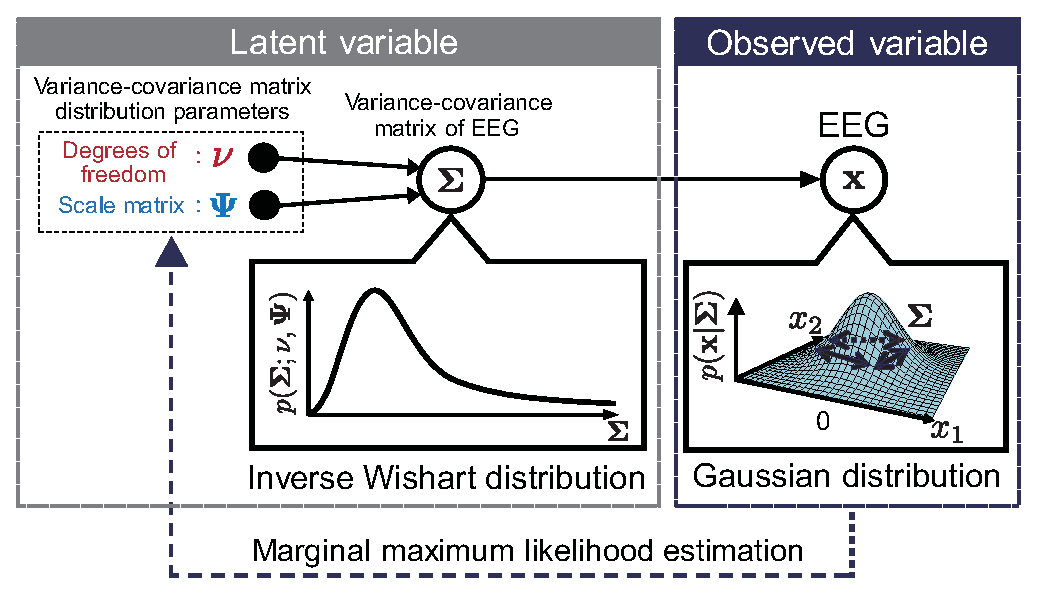
\includegraphics[width=1.0\hsize]{figure/fig1_ver2.eps}
%\end{center}
\caption{Graphical representation of the stochastic relationship between EEG signals  and its variance-covariance matrix.
The white nodes are random variables and the black nodes are parameters to be estimated.
In the model, EEG signals $\mathbf{x}$ are handled as a random variable that follows a multivariate Gaussian distribution with a mean vector of $\mathbf{0}$.
The EEG variance-covariance matrix $\mathbf{\Sigma}$ is also a random variable that follows the inverse Wishart distribution determined by the freedom degree parameter $\nu$ and the scale matrix parameter $\mathbf{\Psi}$.
The variance-covariance matrix distribution parameters are estimated via marginal likelihood maximization from measured EEG signals.}
\label{fig:model}
\end{figure}
%%%%%%%%%%%%%%%%%%%%%%%%%%%%%%%%

まず,分散共分散行列$\bm \Sigma$が与えられた下での脳波$\mathbf{x}$の条件付き分布$P(\mathbf{x}|\mathbf{\Sigma})$は,以下に示す平均ゼロの多変量ガウス分布に従うと考える.
%
\begin{eqnarray}
	p(\mathbf{x}|{\bm \Sigma}) &=& {\mathcal N}(\mathbf{x}|{\bm \Sigma}) \nonumber\\
&=& \frac{1}{(2\pi)^{L/2} |\mathbf{\Sigma}|^{1/2}} \mathrm{exp} \left[-\frac{1}{2}\mathbf{x}^\mathrm{T} {\bm \Sigma}^{-1} \mathbf{x}\right]. \label{eq:gauss_x}
\label{eq:p_x_sigma} %eq1
\end{eqnarray}
%
$\mathbf{\Sigma}$の分布には,多変量ガウス分布の共役事前分布である逆ウィシャート分布${\mathcal {IW}}({\bm \Sigma}; \nu, {\bm \Psi})$を仮定する.
%
\begin{eqnarray}
	p({\bm \Sigma}) &=& {\mathcal {IW}}({\bm \Sigma};\nu,{\bm \Psi}) \nonumber\\
&=& \frac{|{\bm \Psi}|^{\frac{\nu}{2}}}{2^{\frac{\nu L}{2}} \Gamma_L \left(\frac{\nu}{2}\right)} |\bm \Sigma|^{-\frac{\nu+L+1}{2}} \mathrm{exp} \left[-\frac{\mathrm{tr}(\bm \Psi \bm \Sigma^{-1})}{2}\right],\label{eq:p_sigma} %eq2
\end{eqnarray}
%
ここで,$\nu$と${\bm \Psi}$ は逆ウィシャート分布を決定するパラメータであり,$\nu$は分布のガウス性を決定する自由度,${\bm \Psi}$は尺度行列である.いま, $\mathbf{x}$の周辺分布$P(\mathbf{x})$を考えると,
\begin{eqnarray}
	p(\mathbf{x}) &=& \int p({\bm \Sigma})p(\mathbf{x}|{\bm \Sigma}) \mathrm{d}{\bm \Sigma} \nonumber \\
		&=& \int {\mathcal {IW}}({\bm \Sigma}; \nu, {\bm \Psi}) {\mathcal N}(\mathbf{x}|{\bm \Sigma}) \mathrm{d}{\bm \Sigma} \label{eq:marginal_x} \\ %eq3
		&=& \int \frac{|{\bm \Psi}|^{\frac{\nu}{2}}}{2^{\frac{\nu L}{2}} \Gamma_L \left(\frac{\nu}{2}\right)} |\mathbf{\Sigma}|^{-\frac{\nu+L+1}{2}}\mathrm{exp} \left[-\frac{\mathrm{tr}(\bm \Psi \bm \Sigma^{-1})}{2}\right] \nonumber\\
&\quad \times&\frac{1}{(2\pi)^{L/2} |\mathbf{\Sigma}|^{1/2}} \mathrm{exp} \left[-\frac{1}{2}\mathbf{x}^\mathrm{T} {\bm \Sigma}^{-1} \mathbf{x}\right] \mathrm{d}{\bm \Sigma} \nonumber \\
		&=& \frac{|{\bm \Psi}|^{\frac{\nu}{2}}}{2^{\frac{\nu L}{2}} (2\pi)^\frac{L}{2} \Gamma_L \left(\frac{\nu}{2}\right)} \int |\mathbf{\Sigma}|^{-\frac{\nu+L+2}{2}}\nonumber\\
&\quad \times&\mathrm{exp} \left[-\frac{1}{2}\mathrm{tr}\{(\bm \Psi + \mathbf{x} \mathbf{x}^\mathrm{T})\bm \Sigma^{-1}\}\right] \mathrm{d}{\bm \Sigma} \nonumber \\
		%&=& \frac{\Gamma_L(\frac{\nu+1}{2})}{\Gamma_L(\frac{\nu-L+1}{2})} \frac{|\frac{1}{\nu-L+1} {\bm \Psi}|^{-\frac{1}{2}}}{\left[\pi(\nu-L+1)\right]^{\frac{L}{2}}} (1+\Delta)^{-\frac{\nu+1}{2}},
\label{eq:p_x}
&=& \frac{\Gamma(\frac{\nu+1}{2})}{\Gamma(\frac{\nu-L+1}{2})} \frac{|\frac{1}{\nu-L+1} {\bm \Psi}|^{-\frac{1}{2}}}{\left[\pi(\nu-L+1) \right]^{\frac{L}{2}}} (1+\Delta)^{-\frac{\nu+1}{2}} ,%eq4
\end{eqnarray}
%
となる.ただし,$\Delta$はマハラノビス距離の平方で,
%
\begin{eqnarray}
	\Delta &=& \mathbf{x}^\mathrm{T}{\bm \Psi}^{-1}\mathbf{x}.
\end{eqnarray}
%
%%%%%%%%%%%%%%%19/05/05
である.(\ref{eq:gauss_x}),(\ref{eq:marginal_x})式より, $p(\mathbf{x})$ は分散共分散行列が異なる多変量ガウス分布を無限個足し合わせた分布となることがわかる.
以上より,多次元脳波の周辺分布を尺度混合分布によりモデル化することができた.
次小節では,計測した脳波から分散共分散行列のパラメータである$\nu$, $\mathbf{\Psi}$を推定する方法について述べる. %?model?

\subsection{Parameter Estimation Based on Marginal Maximum Likelihood}
%%%%%%%%%%%%%%%19/05/06
いま,$N$サンプルの脳波データ$\mathbf{X} = \{\mathbf{x}_n \in \mathbb{R}^{L}; n=1,2,\cdots,N \}$が観測されたとすると,分散共分散行列分布パラメータ$\nu$, $\bm \Psi$は,周辺分布の尤度$p(\mathbf{X}) = \prod_{n=1}^{N} p(\mathbf{x}_n)$を最大化することで推定できる.
しかしながら,一般に周辺尤度の最尤解は複雑な形となるため,$p(\mathbf{X})$の直接最適化は困難である場合が多い~\cite{t2006}.
そこで本論文では,潜在変数を含むモデルに対する効率的な最適化手法であるEM (expectation-maximization) アルゴリズム\cite{Models1998}に基づいて$\nu$, $\bm \Psi$の推定を行なう.
%%%%%%%%%%%%%%%19/06/12

まず,簡単のため(\ref{eq:p_x})式における分散共分散行列パラメータ$\nu$, $\bm \Psi$を$\nu= \nu' +L-1$, $\bm \Psi = \nu' \bm{\Psi}'$と置き換えると,周辺分布$p(\mathbf{x}_n)$は次のように書き換えることができる.
\begin{align}%ディスプレイ用番号付き6,7
\label{eq:eq6}
p(\mathbf{x}_n) &=\int \mathcal{IW}(\bm{\Sigma}_n; \nu'+L-1, \nu' \bm{\Psi}') \mathcal{N}(\mathbf{x}_n|\bm{\Sigma}_n) \mathrm{d} {\bm{\Sigma}_n} \\
\label{eq:eq7}
&=\frac{\Gamma(\frac{\nu'+L}{2})}{\Gamma(\frac{\nu'}{2})} \frac{|{\bm \Psi'}|^{-\frac{1}{2}}}{\left(\pi \nu' \right)^{\frac{L}{2}}} \left(1+\frac{\Delta '}{\nu '} \right)^{-\frac{\nu'+L}{2}}
\end{align}
ただし,
\begin{eqnarray}
	\Delta ' = \mathbf{x}_n^\mathrm{T} ({\bm \Psi '})^{-1} \mathbf{x}_n
\end{eqnarray}
である.ここで,(7)式はStudentの$t$分布と等価となる~\cite{t2006}.
さらに,EMアルゴリズムに基づく最適化を効率的に行なうため,(\ref{eq:eq6})式を以下の等価な形へと変形する (refer to Appendix).
\begin{equation}%ディスプレイ用番号付き9
\label{eq:eq9}
		p(\mathbf{x}_n) = \int \mathrm{IG}(\tau_n;\nu'/2,\nu'/2) \mathcal{N}(\mathbf{x}_n|\tau_n \mathbf{\Psi}') \mathrm{d}{\tau_n}
\end{equation}
ここで,$\tau_n$は逆ガンマ分布$\mathrm{IG}(\cdot)$に従う確率変数である.この$\tau_n$を潜在変数として再定義し,以下の手順で
周辺尤度が最大となるようなパラメータ$\nu'$, ${\bm \Psi'}$を推定する.
\begin{enumerate}
\setlength{\parskip}{0cm} % 段落間詰める
\setlength{\itemsep}{0cm} % 項目間詰める
\item[(i)] 各パラメータに任意の初期値を与える.
\item[(ii)] Eステップ:完全データ対数尤度$Q(\nu',\bm \Psi')$を計算する.
\begin{align}%ディスプレイ用番号付き10,11
  Q(\nu',\bm{\Psi}')&=\mathbb{E} \left[\ln{\prod_{n=1}^{N}\mathrm{IG}(\tau_n;\nu'/2,\nu'/2) \mathcal{N}(\mathbf{x}_n|\tau_n \bm{\Psi}')}\right]  \notag  \\
  &=\sum_{n=1}^{N} \biggl[-\frac{L}{2}\ln{(2\pi)}-\frac{L}{2}\mathbb{E}\left[\ln{\tau_n}\right]-\frac{1}{2}\ln{|\bm \Psi'|} \notag \\
  &\quad-\frac{1}{2}\mathbb{E}\left[\tau^{-1}_n\right]\Delta'+\frac{1}{2} \ln{\frac{\nu'}{2}} - \ln{\Gamma_L{\left(\frac{\nu'}{2}\right)}} \notag \\
  &\quad- \left(\frac{\nu'}{2}+1\right)\mathbb{E}\left[\ln{\tau_n}\right]+\frac{\nu'}{2}\mathbb{E}\left[\tau^{-1}_n \right] \biggr]
\end{align}
ここで,$\mathbb{E}\left[\tau^{-1}_n\right]$と$\mathbb{E}\left[\ln{\tau_n}\right]$は潜在変数$\tau_n$の事後分布$p(\tau_n|\mathbf{x}_n)$を計算することで以下のように求まる.
\begin{equation}%ディスプレイ用番号付き12
\mathbb{E}\left[\tau^{-1}_n\right]=\frac{\nu'+L}{\nu'+\Delta'}
\end{equation}
\begin{eqnarray}%ディスプレイ用番号付き13
&\mathbb{E}\left[\ln{\tau_n}\right]=-\ln{\mathbb{E}\left[\tau^{-1}_n\right]}+\ln{\left(\frac{\nu+L}{2}\right)}-{\psi}\left(\frac{\nu+L}{2}\right)\quad
\end{eqnarray}
ここで,$\psi(\cdot)$は逆ガンマ関数を表す.
\item[(iii)] Mステップ:$Q(\nu', \bm \Psi')$を最大化することでパラメータを更新する.$Q(\nu', \bm \Psi')$を$\bm \Psi'$で微分しゼロとおくと,新しい尺度行列$\bm \Psi'$は次のように決定される.
\begin{equation}%ディスプレイ用番号付き14
{^\mathrm{new} {\bm \Psi}}' = \frac{1}{N} \sum_{n=1}^{N} \mathbb{E}\left[\tau^{-1}_n\right] \mathbf{x}_n \mathbf{x}_n^\mathrm{T}
\end{equation}
なお,$\nu'$については解析的な解が得られないため,$Q(\nu', \bm \Psi')$を最大化するような$\nu'$の数値解を二分探索によって求める.
\begin{equation}%ディスプレイ用番号付き15
{^\mathrm{new} \nu}' = \argmax_{\nu'}  Q(\nu', {^\mathrm{new} {\bm \Psi}}')
\end{equation}
\item[(iv)] 更新後のパラメータを用いて対数周辺尤度$\ln{p(\mathbf{X})} = \ln{\prod_{n=1}^N p(\mathbf{x}_n)}$を計算し,対数周辺尤度が収束するまで(ii)と(iii)を反復する.
最後に,推定された$t$分布のパラメータである$\nu'$, $\bm \Psi'$を,元の分散共分散行列分布のパラメータ$\nu$, $\bm \Psi$に変換する.
\end{enumerate}
以上の手順より,計測した脳波から分散共分散行列分布のパラメータを推定することができる.
ここで,$\nu$は$t$分布の自由度に対応することから,分布のガウス性を決定するパラメータである.尺度混合モデルの枠組みにおいては,分散に相当するパラメータの確率的変動によって分布のガウス性が変化すると考えることができる.これにより,観測された脳波から$\nu$を推定することで,脳波の分散共分散行列の変動を評価可能となる.

\subsection{Proposed EEG Analysis Methods}
%%%%%%%%%%%%%%%%%%%%%%%%%%%%%%%%
\begin{figure*}[!ht]
\centering
\includegraphics[width=0.95\hsize]{figure/system_2.eps}
%\end{center}
\caption{Overview of the proposed analysis method. The measured EEG signals are decomposed into $\delta$--$\gamma$ frequency band by using filterbank consisting of parallel band pass filters, then the parameter is estimated based on the proposed model and show the results by using color map.}
\label{fig:system}
\end{figure*}
%%%%%%%%%%%%%%%%%%%%%%%%%%%%%%%%
Fig. \ref{fig:system}に,提案する脳波解析手法の概略図を示す.
提案法では,観測した脳波をバンドパスフィルタの並列によって構成されるフィルタバンクを用いて複数の周波数帯域に分解する.
そして,各帯域の信号に対して尺度混合モデルに基づく確率的変動の推定を行なう.

まず,$L$対の電極から計測された時刻$t$における脳波を$\mathbf{x}_t \in \mathbb{R}^L$とする.そして,$\mathbf{x}_t$に対して3次のバタワースバンドパスフィルタによって構成されたフィルタバンクを適用することで,信号を$f_n$個の周波数帯域に分解し,得られた信号を$\mathbf{x}^{(f_n)}_t$とする.
$\delta$ (1--3 Hz), $\theta$ (4--7 Hz), $\alpha$ (8--12 Hz), $\beta$ (13--24 Hz), $\gamma$ (25--100 Hz) の5つの周波数帯域に分解し,得られた信号を$\mathbf{x}^{(f)}_t$ ($f \in\{\delta, \theta, \alpha,\beta, \gamma\}$)とする.なお,これらの周波数帯域は脳波の特性をとらえるために一般的に用いられているものである~\cite{ep1994}.
次に,$\mathbf{x}^{(f)}_t$に対して周波数帯域ごとに尺度混合モデルに基づく分散共分散行列分布のパラメータ推定を行ない,確率的変動を特徴付ける$\nu$を取得する.ここで,脳波は時系列に特性が大きく変化する信号であるため,各帯域の信号$\mathbf{x}^{(f)}_t$に対して幅$W$ [s]の移動窓を適用し,窓内のサンプルに対してII--\textit{B}.の手順に基づきパラメータ$\nu$を推定する.この移動窓を$S$ [s]ずつスライドさせながら連続的に推定を行なうことで,時系列に$\nu$の推定結果を取得可能である.ここで,$\nu$は$\infty$に近くなるほど分布がガウス分布に近づく,つまり確率的変動が小さくなることを意味するパラメータである.そこで本論文では,$\nu$の逆数である$1/\nu$を算出し,これを確率的変動を特徴付ける指標として用いる.この$1/\nu$は,値が大きいほど脳波の確率的変動が大きいことを示す.

以上より,脳波の各帯域に潜在する確率的変動を時系列に取得することができる.
また,事前に脳波の電極配置を複数の領域に分割しておき,領域ごとに上記の解析を行なうことで,確率的変動の空間分布を取得することも可能である.
\section{Experiments}
\subsection{Patients}
被験者は,専門医によって焦点発作と診断されたてんかん患者20名 (Table \ref{table:conditions}参照)であり,頭皮表面に貼付した電極からサンプリング周波数$f_\mathrm{s} = 500$ Hzで脳波を計測した.電極数は19対 ($L=19$) とし,電極位置は国際10--20法に基づいて決定した (Fig. \ref{fig:electrodes}参照) .脳波の導出には,耳朶の電極であるA1,A2を基準電極として設定する単極誘導法を用いた.なお,本論文における解析は岡山大学生命倫理委員会の承認のもと実施した (承認番号:研1706-019).


%%%%%%%%%%%%%%%%%%%%%%%%%%%%%%%%
\begin{figure}[!t]
\centering
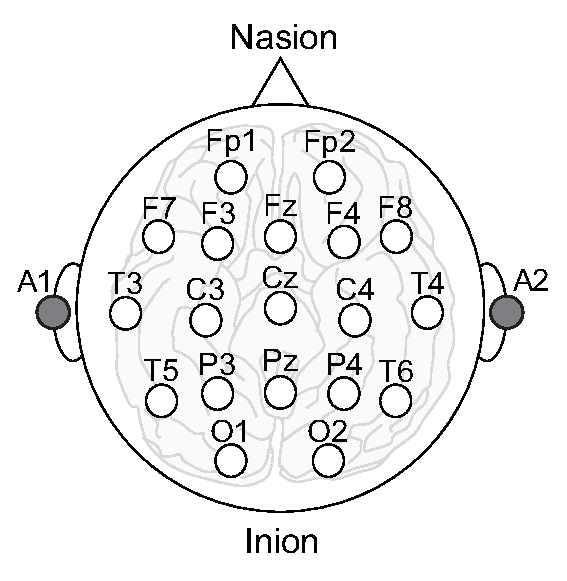
\includegraphics[width=0.6\hsize]{figure/electrodes.eps}
%\end{center}
\caption{International 10--20 electrode montage.}
\label{fig:electrodes}
\end{figure}
%%%%%%%%%%%%%%%%%%%%%%%%%%%%%%%%

%=====================
%Table1 被験者
%=====================
\begin{table}[t]
 \begin{center}
 \caption[Subject conditions]{Subject conditions}
 \label{table:conditions}
 \vspace{-2.5mm}
% \scalebox{0.86}[0.86]{%size
  \begin{tabular}{ccccc}
   \toprule %booktabs
   \multirow{2}{*}{Subject} &  \multirow{2}{*}{Sex} &  Age  & Total data & Seizure duration \\
   & & [year] &  length [s] & [s] \\
   \midrule %booktabs
   Sub. A & Male & 2 & 300 & 71\\ %AS
   Sub. B & Male & 23 & 300 & 54\\ %ZX
   Sub. C & Male & 2 & 300 & 71\\ %AR
   Sub. D & Male & 4 & 380 & 93\\ %IP
   Sub. E & Female & 31 & 320  & 39\\ %IQ
   Sub. F & Male & 0.5 & 500 & 158\\ %IS省くかも20190716 20190918省く!!
   Sub. G & Female & 14 & 420 & 72\\ %IT省くかも20190716 20190918省く!!
   Sub. H & Male & 19 & 390 & 36\\ %IV
   Sub. I & Male & 0.8 & 360  & 98\\ %15
   Sub. J & Male & 20 & 390 & 16\\ %IW
   Sub. K & Male & 36 & 300 & 23\\ %NR
   Sub. L & Male & 9 & 300 & 43\\ %NS
   Sub. M & Male & 13 & 300  & 43\\ %ZR
   Sub. N & Male & 12 & 300 & 88\\ %ZS
   Sub. O & Male & 8 & 300 & 17\\ %ZT
   Sub. P & Female & 19 & 300 & 69\\ %ZV
   Sub. Q & Male & 27 & 420 & 62\\ %AB
	 Sub. R & Male & 38 & 300 & 65\\ %ZY
	 Sub. S & Male & 17 & 300 & 17\\ %ZZ
	 Sub. T & Male & 19 & 300 & 65\\ %00
   \bottomrule %booktabs
  \end{tabular}
 \end{center}
\end{table}

%=====================
\subsection{Experiment I (Estimate parameter) }
提案モデルが脳波の確率的変動を捉えているかを検証するため,多変量t分布を用いて,疑似脳波をあるサンプル数だけ乱数生成し,推定値と実測値の誤差を確認するシミュレーション実験を行なった.
解析には,多変量t分布の二つのパラメータ自由度$\nu$,尺度行列$\mathbf{\Psi}$を固定し,サンプル数を~~,--,||まで変更させた19次元のデータを用いることで,誤差が最小となるサンプル数を探索した.
誤差の評価には,推定値と実測値の差の絶対値である絶対誤差を算出した.
\begin{equation}%ディスプレイ用番号付き12
		\mathrm{Absolute\;error} = |\mathrm{(estimated\;value)}-\mathrm{(true\;value)}|
\end{equation}

\subsection{Experiment II (Epileptic EEG analysis)}
提案法に基づく脳波の確率的変動評価の有効性を検証するため,てんかん発作時の脳波に対して解析を行なった.

提案法に基づく解析には,計測したデータから切り出した発作前後の一定時間のデータを使用した.
各被験者の情報,解析に用いた時間,および発作持続時間を Table \ref{table:conditions}に示す.
解析時の移動窓幅の大きさ$W$およびそのずらし幅$S$は,専門医の知見に基づきそれぞれ$W = 10$ s ,$S = 1$ sとした.

提案法により算出した各帯域の$1/\nu$を用いて,てんかん発作/非発作の分類性能を評価した.まず,各被験者における$1/\nu$の算出結果を,発作区間から得られたものと非発作区間から得られたものに分割した.ここで,非発作区間は解析開始から発作が生じるまでと定義しており,元の脳波において体動や電極シフトなどによるノイズの影響が顕著に見られた区間は対象から除外した.また,発作区間と非発作区間で$1/\nu$のサンプル数が大きく異なるため,発作区間のサンプル数を基準として非発作区間から抽出し,被験者ごとに$1/\nu$のサンプル数を揃えた.

分類性能の評価は,ROC解析 (receiver operating characteristic analysis) に基づき算出したROC曲線下面積(area under the curve : AUC)を用いて行なった.ここで,AUCとは偽陽性率と真陽性率との関係をプロットしたROC曲線から算出される評価尺度であり,値が1に近いほど識別性能が高いことを表す.また比較として,脳波の振幅情報のみを用いて同様にAUCの算出を行なった.振幅情報には,以下の式で表されるRMS (root mean square)を用いた\cite{Hamedi2014}.
\begin{equation}%ディスプレイ用番号付き12
		\mathrm{RMS} = \sqrt{\frac{1}{N_W} \sum_{i=1}^{N_W} (x_i^\mathrm{Cz})^2}
\end{equation}
ここで,$x_i^\mathrm{Cz}$は頭頂部のチャネルCzから得られた脳波,$N_W$は移動窓内のサンプル数である.このRMSを$1/\nu$の算出時と同じ窓幅$W = 10$ s,ずらし幅$S = 1$ sで連続的に算出した.

\section{Results}
\subsection{Experiment 1(estimate parameter)}
観測した非発作と発作時脳波の分布の違いを解析するために,パラメータの推定実験を行なった.解析に用いた脳波は被験者2名の10秒間のデータであり,それぞれ非発作と発作時の脳波に対して提案モデルと従来のガウスモデル,ラプラスモデルを用いてフィッティングを行なった結果をFig. \ref{fig:hist}に示す.Fig. \ref{fig:window}には,移動窓幅を変更させた際の各帯域のAUCの変化を示している.

\subsection{Experiment 2 (Epileptic EEG analysis)}
Fig. \ref{fig:Colormap}に,Sub. A, Sub. Bにおける脳波の生波形と対応する$1/\nu$の算出結果をカラーマップにより示す.
本カラーマップにおいて,1/$\nu$は全帯域の最大値が1となるように正規化している.
なお,波形中の陰影部およびカラーマップ中の白点線で示している箇所は,専門医がてんかん発作と診断した区間である.

Fig. \ref{fig:dens}に,カーネル密度推定~\cite{Parzen1962}により算出した全被験者に対する各帯域の$1/\nu$の分布を,発作区間と非発作区間のそれぞれについて示す.
図中にはBonferroni-Holm調整を用いた対応ありWilcoxon符号付き順位検定 (有意水準:1\%)の結果と効果量$g$~\cite{Hedges1981}を併記している.
ここで,効果量$g$とは2つの分布の平均値の差の大きさを表す統計的指標であり,一般的に$0.2 \leq g < 0.5$は小さな効果量,$0.5 \leq g < 0.8$は中程度の効果量,$0.8 \leq g$は大きな効果量と解釈される.
Fig. \ref{fig:roc}(a)に,発作/非発作の分類によって得られたROC曲線を,各帯域における$1/\nu$と振幅情報であるRMSのそれぞれについて示す.またこのROC曲線から得られたAUCをFig. \ref{fig:roc}(b)に示す.各帯域 ($\delta$--$\gamma$)における$1/\nu$のAUCはそれぞれ, 0.657, 0.597, 0.605, 0.757, 0.868となり,RMSのAUCは0.847となった.

%%%%%%%%%%%%%%%%%%%%%%%%%%%%%%%%
\begin{figure}[!t]
\centering
\includegraphics[width=0.9\hsize]{figure/Colormap.eps}
%\end{center}
\caption{Analysis results of the proposed method for (a)Sub. A and (b)Sub. B.}
\label{fig:Colormap}
\end{figure}
%%%%%%%%%%%%%%%%%%%%%%%%%%%%%%%%

%%%%%%%%%%%%%%%%%%%%%%%%%%%%%%%%
\begin{figure}[!t]
\centering
\includegraphics[width=0.9\hsize]{figure/ROC_rms.eps}
%\end{center}
\caption{Results of $1/\nu$ for each frequency band and RMS. (a)ROC curves. (b)AUCs. }
\label{fig:roc}
\end{figure}
%%%%%%%%%%%%%%%%%%%%%%%%%%%%%%%%

%%%%%%%%%%%%%%%%%%%%%%%%%%%%%%%%
\begin{figure}[!t]
\centering
\includegraphics[width=0.95\hsize]{figure/window_w50.eps}
%\end{center}
\caption{Results of AUCs for each frequency band by changing window length. }
\label{fig:window}
\end{figure}
%%%%%%%%%%%%%%%%%%%%%%%%%%%%%%%%

\section{Discussion}
%-------------------
%考察
%-------------------
Fig. \ref{fig:Colormap}より,てんかん発作区間において特に高周波帯域の$1/\nu$が大きくなっていることがわかる.
この傾向は,全ての被験者に共通して確認することができた.このことから,提案法を用いることで,てんかん発作に伴う脳波の非ガウス性の変化を確率的変動として定量的に評価できていると考えられる.

Fig. \ref{fig:dens}より,全被験者の各帯域における$1/\nu$の分布を確認すると,非発作時の$1/\nu$は帯域によらず0.25未満の領域に分布していることがわかる.一方,発作時の$1/\nu$は非発作時よりも広く分布しており,その傾向は高周波になるにつれ強くなっていることがわかる.これは平均値の差の程度を表す効果量$g$の結果からも確認できる.$\beta$や$\gamma$帯域において大きな効果量が得られたことから,高周波帯域における$1/\nu$がてんかん発作時の特徴を最も反映していると考えられる.これは,てんかん発作に伴い脳波の高周波帯域が強い非ガウス性を示したことを意味している.てんかん発作時に脳波の高周波帯域である$\gamma$帯域の活動が活発になることは従来研究においても報告されている~\cite{Kobayashi2004,Kobayashi2009,Benedek2016}.その詳しいメカニズムはいまだ明らかにされていないものの,皮質と皮質下構造の間の複雑な相互作用に起因すると考えられている~\cite{Kobayashi2004}.この相互作用の異常によっててんかん発作時特有の断続的な振幅変化が生じ,結果として高周波帯域の非ガウス性が強調され$1/\nu$が増加した可能性がある.

Fig. \ref{fig:roc}(b)より,各帯域における$1/\nu$のAUCを確認したところ,高周波帯域である$\gamma$帯域で0.868と中程度ながら高い値が得られており,$\gamma$帯域の$1/\nu$が最も分類性能が高いことがわかる.また,従来の特徴量であるRMSと比較したところ,$\gamma$帯域の$1/\nu$は従来法と同程度以上の識別性能を有することが示された.振幅の絶対的な大きさであるRMSと,提案法から算出される$1/\nu$は脳波活動の異なる側面を捉えていると考えられるため,今後はこれらを組み合わせることでより高い識別性能を獲得できる可能性がある.

\section{Conclusion}
以上より,提案法を用いて,てんかん発作に伴う脳波の確率的変動を定量的に評価することができ,この特徴変化を用いることでてんかん発作検出へと応用できる可能性が示された.
しかしながら,Fig. \ref{fig:Colormap}(a)の220 s付近を見ると,てんかん発作以外の区間においても部分的な$1/\nu$の増加が認められた.これは,筋電位などの高周波帯域のアーティファクトにより確率的変動が大きくなったためであると考えられるため,専門医の知見に基づき,解析結果についてより詳細に検討していく必要がある.
今後は,逆ウィシャート分布のもう一つのパラメータである$\mathbf{\Psi}$の評価や筋電位などのアーティファクトの除去などを行なう予定である.


\appendix[Equivalent calculation on Scale mixture model]
(\ref{eq:eq6})式と(\ref{eq:eq9})式が等価であることを以下に示す.
\begin{eqnarray}
	&p(\mathbf{x}_n) \nonumber\\ &=& \int \mathrm{IG}(\tau_n;\nu'/2,\nu'/2) \mathcal{N}(\mathbf{x}_n|\tau_n \mathbf{\Psi}') \mathrm{d}{\tau_n} \nonumber\\
	&=& \int \frac{\left(\frac{\nu'}{2}\right)^{\frac{\nu'}{2}}}{\Gamma \left(\frac{\nu'}{2}\right)} (\tau_n)^{-\frac{\nu'}{2}-1} \mathrm{exp} \left[-\frac{1}{\tau_n} \left(\frac{\nu'}{2} \right) \right] \nonumber\\
	&\quad\times&\frac{1}{(2\pi)^{\frac{L}{2}}(\tau_n)^{\frac{L}{2}}|\mathbf{\Psi'}|^{\frac{1}{2}}} \mathrm{exp} \left[-\frac{1}{2}\mathbf{x}^\mathrm{T} (\tau_n\mathbf{\Psi'})^{-1} \mathbf{x}\right] \mathrm{d}{\tau_n} \nonumber\\
	&=&\frac{1}{(2\pi)^{\frac{L}{2}}}\frac{\left(\frac{\nu'}{2}\right)^{\frac{\nu'}{2}}}{\Gamma \left(\frac{\nu'}{2}\right)}\frac{1}{|\mathbf{\Psi'}|^{\frac{1}{2}}} \nonumber\\
	&\quad\times& \int (\tau_n)^{-\frac{\nu'+L}{2}-1} \mathrm{exp} \left[-\frac{1}{\tau_n} \left(\frac{\nu' + \Delta'}{2}\right) \right] \mathrm{d}{\tau_n} \nonumber\\
	&=&\frac{1}{(2\pi)^{\frac{L}{2}}}\frac{\left(\frac{\nu'}{2}\right)^{\frac{\nu'}{2}}}{\Gamma \left(\frac{\nu'}{2}\right)}\frac{1}{|\mathbf{\Psi'}|^{\frac{1}{2}}} \frac{\Gamma \left(\frac{\nu'+L}{2}\right)}{\left(\frac{\nu'+\Delta'}{2}\right)^{\frac{\nu'+L}{2}}}\nonumber\\
	&\quad\times& \int \frac{\left(\frac{\nu'+\Delta'}{2}\right)^{\frac{\nu'+L}{2}}}{\Gamma \left(\frac{\nu'+L}{2}\right)} (\tau_n)^{-\frac{\nu'+L}{2}-1} \nonumber\\
	&\quad\times& \mathrm{exp} \left[-\frac{1}{\tau_n} \left(\frac{\nu' + \Delta'}{2}\right) \right] \mathrm{d}{\tau_n} \nonumber\\
	&=&\frac{1}{(2\pi)^{\frac{L}{2}}}\frac{\left(\frac{\nu'}{2}\right)^{\frac{\nu'}{2}}}{\Gamma \left(\frac{\nu'}{2}\right)}\frac{1}{|\mathbf{\Psi'}|^{\frac{1}{2}}} \frac{\Gamma \left(\frac{\nu'+L}{2}\right)}{\left(\frac{\nu'+\Delta'}{2}\right)^{\frac{\nu'+L}{2}}}\nonumber\\
	&\quad\times& \int \mathrm{IG}(\tau_n;\frac{\nu'+L}{2},\frac{\nu'+\Delta'}{2}) \mathrm{d}{\tau_n}\nonumber\\
	&=& \frac{\Gamma(\frac{\nu'+L}{2})}{\Gamma(\frac{\nu'}{2})} \frac{|{\bm \Psi'}|^{-\frac{1}{2}}}{\left(\pi \nu' \right)^{\frac{L}{2}}} \left(1+\frac{\Delta '}{\nu '} \right)^{-\frac{\nu'+L}{2}}.
\end{eqnarray}

% if have a single appendix:
%\appendix[Proof of the Zonklar Equations]
% or
%\appendix  % for no appendix heading
% do not use \section anymore after \appendix, only \section*
% is possibly needed

% use appendices with more than one appendix
% then use \section to start each appendix
% you must declare a \section before using any
% \subsection or using \label (\appendices by itself
% starts a section numbered zero.)
%



% use section* for acknowledgment
%\section*{Acknowledgment}


%The authors would like to thank...


% Can use something like this to put references on a page
% by themselves when using endfloat and the captionsoff option.
\ifCLASSOPTIONcaptionsoff
  \newpage
\fi



% trigger a \newpage just before the given reference
% number - used to balance the columns on the last page
% adjust value as needed - may need to be readjusted if
% the document is modified later
%\IEEEtriggeratref{8}
% The "triggered" command can be changed if desired:
%\IEEEtriggercmd{\enlargethispage{-5in}}

% references section

% can use a bibliography generated by BibTeX as a .bbl file
% BibTeX documentation can be easily obtained at:
% http://mirror.ctan.org/biblio/bibtex/contrib/doc/
% The IEEEtran BibTeX style support page is at:
% http://www.michaelshell.org/tex/ieeetran/bibtex/
%\bibliographystyle{IEEEtran}
% argument is your BibTeX string definitions and bibliography database(s)
%\bibliography{IEEEabrv,../bib/paper}
%
% <OR> manually copy in the resultant .bbl file
% set second argument of \begin to the number of references
% (used to reserve space for the reference number labels box)

\bibliographystyle{IEEEtran}
\bibliography{ref.bib}


% You can push biographies down or up by placing
% a \vfill before or after them. The appropriate
% use of \vfill depends on what kind of text is
% on the last page and whether or not the columns
% are being equalized.

%\vfill

% Can be used to pull up biographies so that the bottom of the last one
% is flush with the other column.
%\enlargethispage{-5in}



% that's all folks
\end{document}
